\documentclass{beamer}

\usepackage{amsmath}
\usepackage{amsfonts}
\usepackage{graphicx}
\usepackage{blindtext}
\usepackage{caption}


\usetheme{Execushares}

\title{Optimal Trajectory Exploration: Thrust Vectored Wing}
\subtitle{Final Project ECEN 5008}
\author{Zachary Vogel\quad Ben Schroeder}% Chris Gavin\and Topher Pollard}
\date{\today}

\setcounter{showSlideNumbers}{1}

\begin{document}
    
    \setcounter{showProgressBar}{0}
    \setcounter{showSlideNumbers}{0}
    
    
    \frame{\titlepage}
    
    \setcounter{framenumber}{0}
    \setcounter{showProgressBar}{1}
    \setcounter{showSlideNumbers}{1}
    
    \section{Introduction}
    \begin{frame}
        \frametitle{Topic}
        \begin{columns}[c]
            \begin{column}{0.6\textwidth}
                \begin{itemize}
                    \item A wing with a magical hand of god thrust on the back
                    \item Examining in two dimensions, x and z, assume no change in y
                    \item Want to fly around a figure eight in these two dimensions
                    \item Also important to be able to transistion between equillibriums
                \end{itemize}
            \end{column}
            \begin{column}{0.4\textwidth}
                \begin{figure}
                    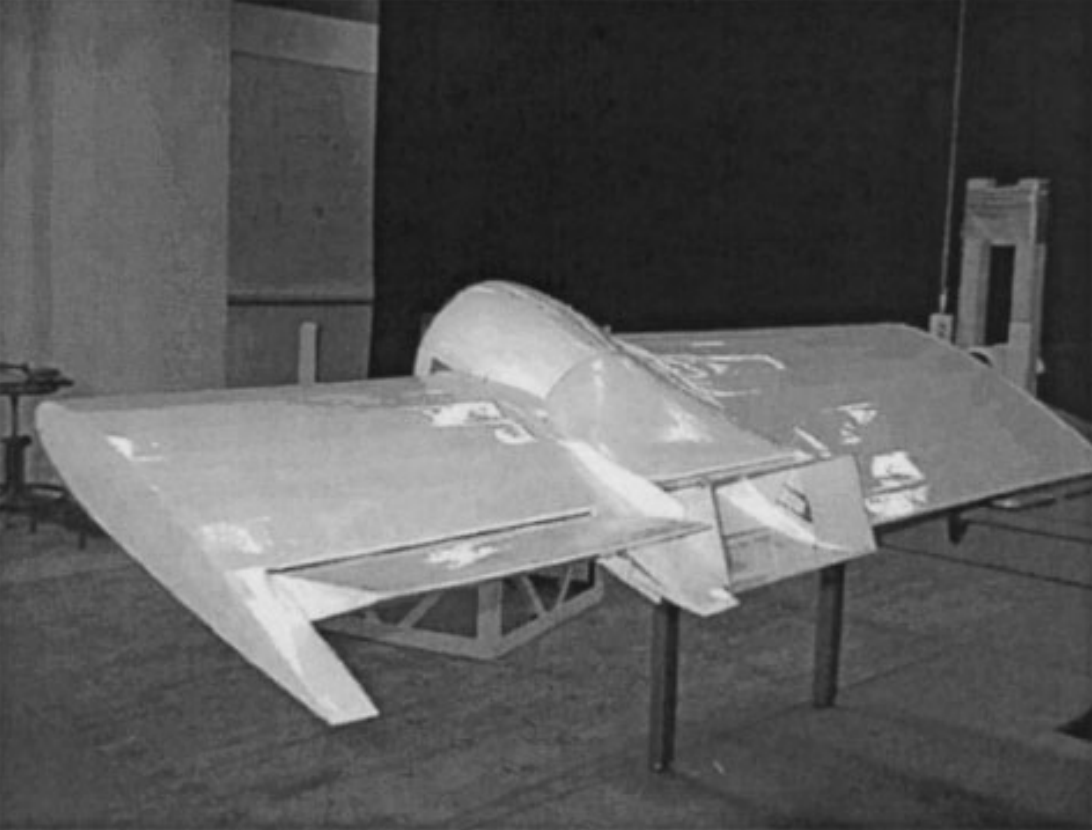
\includegraphics[width=0.95\textwidth]{ducted_fan.png}
                    \caption*{Caltech Ducted Fan}
                \end{figure}
            \end{column}
        \end{columns}
    \end{frame}
    
    \section{Background}
    \begin{frame}
        \frametitle{Model}
        \begin{columns}[c]
            \begin{column}{0.6\textwidth}
                \begin{itemize}
                    \item Angle of attack $\alpha$, $\theta$ is plane angle from x axis
                    \item Thrust vector in x and z applied to a point on towards the back of the plane
                    \item Lift perpendicular to Velocity, Drag parallel to velocity
                    \item Mathematics done in the Velocity frame
                    \item Constants pulled straight from references
                \end{itemize}
            \end{column}
            \begin{column}{0.4\textwidth}
                \begin{figure}
                    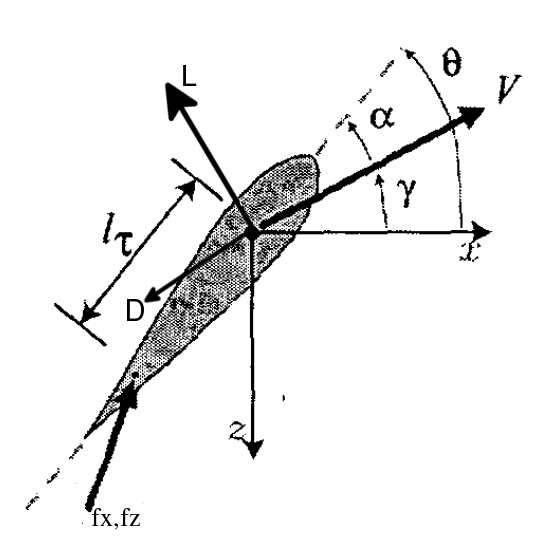
\includegraphics[width=0.95\textwidth]{wing_model.png}
                    \caption*{Basic model of the Thrust Vectored Wing}
                \end{figure}
            \end{column}
        \end{columns}
    \end{frame}

    \begin{frame}
        \frametitle{Final Dynamics}
        \[\dot{v}=-\frac{D(v,\alpha)}{m}-g\sin(\theta-\alpha)+\frac{\cos(\alpha)}{m}f_x+\frac{\sin(\alpha)}{m}f_z\]
        \[\dot{\alpha}=-\frac{L(v,\alpha)}{mv}+\frac{g}{v}\cos(\theta-\alpha)-\frac{\sin(\alpha)}{mv}f_x+\frac{\cos(\alpha)}{mv}f_z\]
        \[\dot{\omega}=\frac{M(v,\alpha)}{J}+\frac{l_{\tau}}{J}f_z\]
        \[\dot{\theta}=\omega\]
        \[\dot{x}=v\cos(\gamma)\quad \dot{z}=-v\sin(\gamma)\]
    \end{frame}
    \begin{frame}
        \frametitle{Lift, Drag and Moment}
        \[L(V,\alpha)=\frac{1}{2}\rho V^2 SC_l(\alpha)\quad D(V,\alpha)=\frac{1}{2}\rho V^2SC_D(\alpha)\]
        \[M(V,\alpha)=\frac{1}{2}\rho V^2S\bar{c}C_m(\alpha)\]
        \[C_l(\alpha)=C_{l_\alpha}\alpha=3.256\alpha\]
        \[C_d(\alpha)=C_{C_{d_0}}+C_{d_\alpha}\alpha^2=0.1716+2.395\alpha^2\]
        \[C_M(\alpha)=C_{M_\alpha}\alpha=-0.0999\alpha\]
        \[S=0.6 \text{m}^2,\quad \rho=1.2 \text{kg/m}^3,\quad J=0.25 \text{kg m}^2\]
        \[l_\tau=0.31\text{m},\quad m=12\text{kg},\quad g=0.6\text{m/s}^2\]
    \end{frame}

    
    \section{Implementation}
    \begin{frame}
        \frametitle{Comparison to Sliding Car}
        \begin{itemize}
            \item One extra state compared to the sliding car
            \item Here the moment is coupled to the thrust and aerodynamic forces
            \item The $\theta$ state exists because of gravity ($g_p=0.6 m/s^2$)
            \item Angle of attack is similar to side slip angle
        \end{itemize}
    \end{frame}

    \begin{frame}
        \frametitle{Coding and Derivatives}
        \begin{itemize}
            \item We already took all the Jacobian and Hessian derivatives
            \item This is where we saw further effects of coupling with more second order derivatives being non-zero
            \item For now, we ignore these second order terms
            \item We trim around a fixed velocity and $\gamma$
            \item We used a partition of unity with the hyberbolic tangent function to transfer from one trim trajectory to another
            \item To get the flight path we integrated the kinematics of shown above
        \end{itemize}
    \end{frame}


    \section{Results}
    \begin{frame}
        \frametitle{Constant Gain Control}
        \framesubtitle{Gamma}
        \begin{figure}
            \centering
            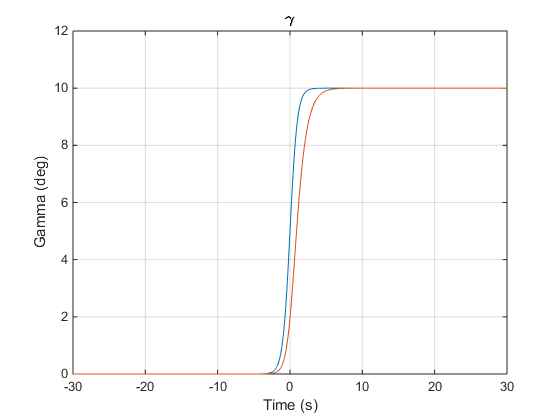
\includegraphics[width=0.9\textwidth]{gamma.png}
        \end{figure}
    \end{frame}

    \begin{frame}
        \frametitle{Velocity}
        \begin{figure}
            \centering
            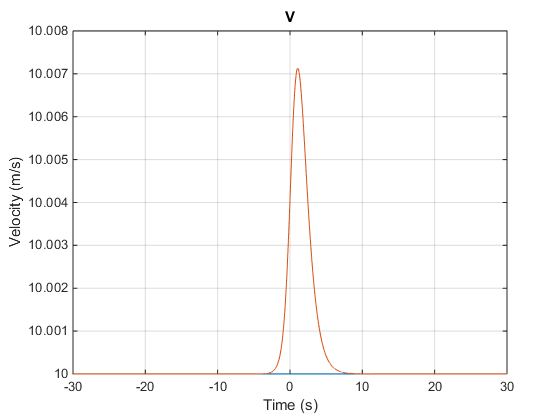
\includegraphics[width=0.9\textwidth]{velocity.png}
        \end{figure}
    \end{frame}
    \begin{frame}
        \frametitle{u2}
        \begin{figure}
            \centering
            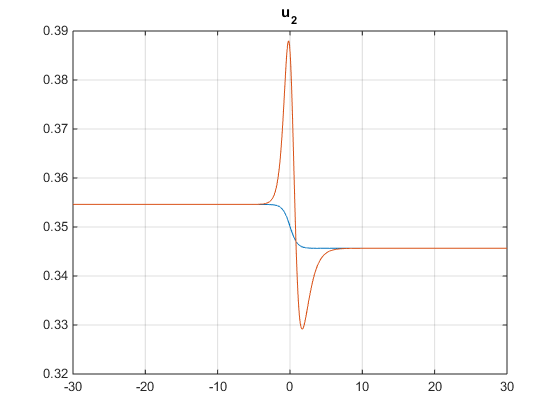
\includegraphics[width=0.9\textwidth]{u2.png}
        \end{figure}
    \end{frame}
    \begin{frame}
        \frametitle{Flight Path}
        \begin{figure}
            \centering
            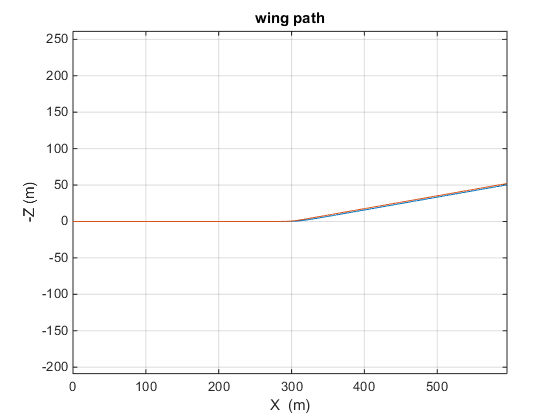
\includegraphics[width=0.9\textwidth]{Flightpath.png}
        \end{figure}
    \end{frame}



    \begin{frame}
        \frametitle{Optimized Time-Varying Control}
        \framesubtitle{Alpha}
        \begin{figure}
            \centering
            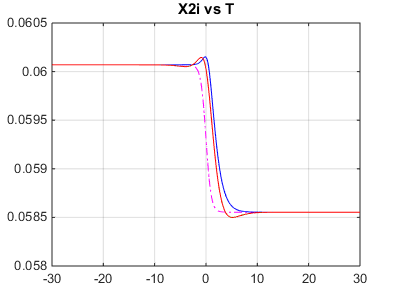
\includegraphics[width=0.9\textwidth]{alpha_it.png}
        \end{figure}
    \end{frame}
    
    \begin{frame}
        \frametitle{Omega}
        \begin{figure}
            \centering
            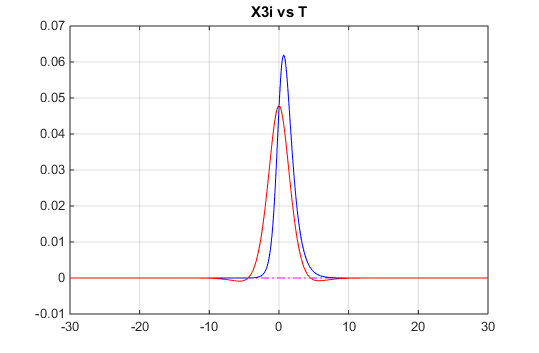
\includegraphics[width=0.9\textwidth]{omega_it.png}
        \end{figure}
    \end{frame}

    \begin{frame}
        \frametitle{Velocity}
        \begin{figure}
            \centering
            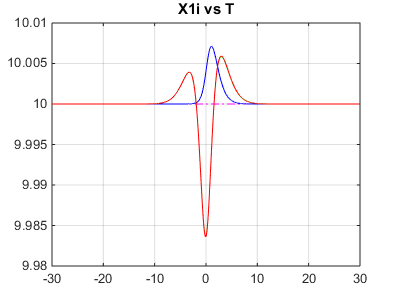
\includegraphics[width=0.9\textwidth]{velocity_it.png}
        \end{figure}
    \end{frame}
    
    \begin{frame}
        \frametitle{Flight Path}
        \begin{figure}
            \centering
            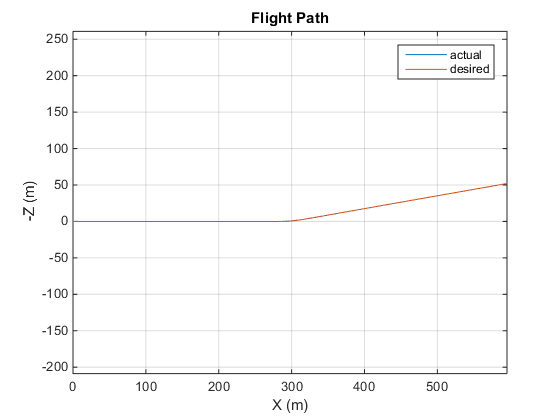
\includegraphics[width=0.9\textwidth]{flight_path_optimal.png}
        \end{figure}
    \end{frame}
    
    \begin{frame}
        \frametitle{First Part of Figure Eight}
        \begin{figure}
            \centering
            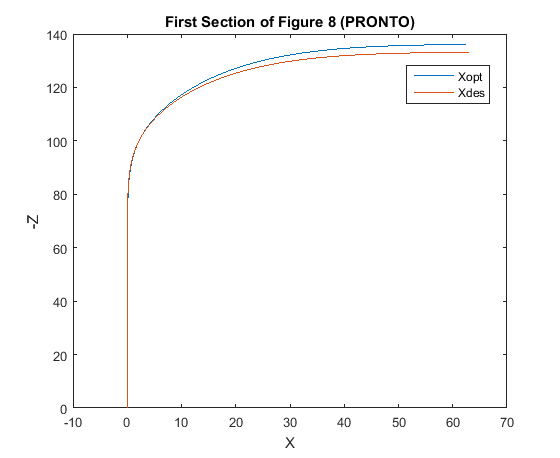
\includegraphics[width=0.8\textwidth]{first_section.png}
        \end{figure}
    \end{frame}
    \begin{frame}
        \frametitle{With Weighting}
        \begin{figure}
            \centering
            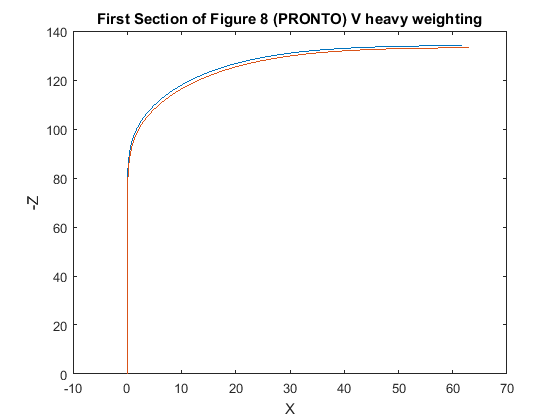
\includegraphics[width=0.8\textwidth]{first_section_weight.png}
        \end{figure}
    \end{frame}
    \begin{frame}
        \frametitle{Constant Gain Descent}
        \begin{figure}
            \centering
            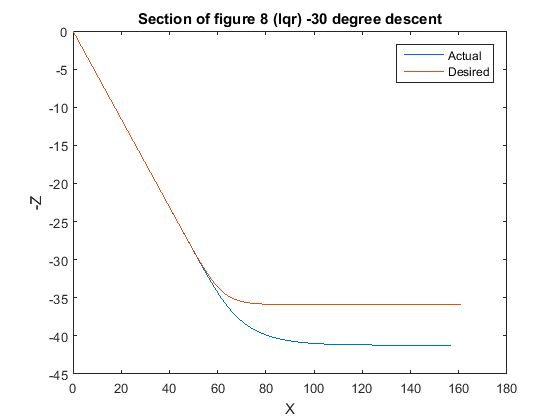
\includegraphics[width=0.8\textwidth]{fig_descent_constant.png}
        \end{figure}
    \end{frame}
    \begin{frame}
        \frametitle{Low Velocity Figure 8 Section}
        \begin{figure}
            \centering
            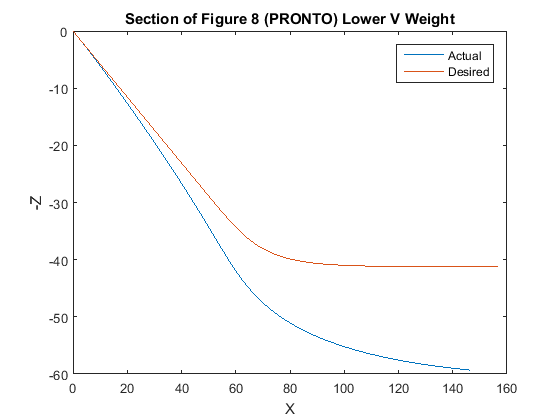
\includegraphics[width=0.8\textwidth]{fig8_rightlow.png}
        \end{figure}
    \end{frame}

    \begin{frame}
        \frametitle{Optimal Descent Heavy Weight}
        \begin{figure}
            \centering
            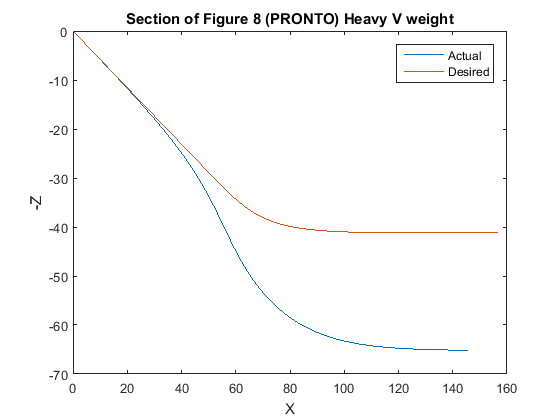
\includegraphics[width=0.8\textwidth]{opt_descent_HW.png}
        \end{figure}
    \end{frame}

    \section{Conclusion}
    \begin{frame}
        \frametitle{Concluding Points}
        \begin{itemize}
            \item Tracked velocities close to 10 well, but anything over 12 failed to converge
            \item Descent overshot every time (Thus we crash into the ground)
            \item Final figure 8 won't be perfect clothoid figure 8
            \item Certain weights made optimization fail 
        \end{itemize}
    \end{frame}

    \begin{frame}
        \frametitle{Further Work}
        \begin{itemize}
            \item Cuban Eight Trajectory
            \item Fix trajectory tracking, especially on the descent
            \item Include second order terms?
            \item Make sure optimization gives best results
        \end{itemize}
    \end{frame}

    \begin{frame}
        \frametitle{Questions?}
        \begin{figure}
            \centering
            
\includegraphics[width=0.7\textwidth]{seal.jpg}
            \caption*{Ben does not approve of this pictures}
        \end{figure}
    \end{frame}

    \begin{frame}[allowframebreaks]
        \frametitle{References}    
        \begin{thebibliography}{10}    
            \beamertemplatearticlebibitems
            \bibitem{Hauser2002}
            J.~Hauser, A.~Jadbabaie
            \newblock {\em Aggressive Maneuvering of a Thrust Vectored Flying Wing: A Receding Horizon Approach}.
            \newblock {\em International Journal of Robust and Nonlinear Control}, 12:869--896. doi:10.1002/rnc.708
            \beamertemplatearticlebibitems
            \bibitem{Hauser2003}
            R.~Franz, J.~Hauser
            \newblock {\em Optimization Based Parameter Identification fo the Caltech Ducted Fan}
            \newblock {\em Proceedings of the 2003 American Control Conference}, 2697--2702, 2003.
        \end{thebibliography}
    \end{frame} 

\end{document}
